\chapter{Input Subsidies to Increase Food Security}
\chapterauthor{Koen Leuveld, Eleonora Nillesen, Janneke Pieters, Martha Ross, Maarten Voors and Elise Wang Sonne}
\label{chap:n2a_impact}

\renewcommand{\thetable}{\arabic{chapter}.\arabic{table}}


\begin{abstract}
We use a field experiment to test the impact of a one-off input subsidy program for a sample of smallholders in Eastern DRC. To date, studies on the topic are typically concentrated in areas where use of the subsidized input is common, which raises the question whether results are generalizable to settings where input use is very limited, yet adoption may be warranted. We investigate the impact of input subsidies in Eastern DRC, arguably among the poorest and unstable regions of the world, where farmers face daily threats of (extreme) violence and displacement, and prior use of fertilizer or other advanced agricultural technologies has been exceptionally low. We find robust evidence for impacts on input use at the extensive margin, one year after the subsidy program: providing subsidies increases fertilizer use by five percentage points, while use of inoculant increases by three percentage points. These effects are substantial given very low use rates in villages without the subsidy program. We measure impacts two agricultural seasons after the subsidy program, suggesting effects persist beyond the season in which the subsidized inputs were offered. Higher input use however does not translate into higher yields in our sample, nor does it affect food security. Moreover, input use was not affected in villages further away from input markets, suggesting that time and costs associated with accessing inputs restrict the impact of subsidy interventions in a context like Eastern DRC.  
\end{abstract}

\section{Introduction} 
Smallholder farmers in sub-Saharan Africa face acute constraints to productivity. Output prices are low, input costs are high, and credit markets function poorly, resulting in low adoption rates of new technologies \citep{Morris2007,Sheahan2014}. Input subsidization programs have recently been reintroduced to address constraints of high input prices, and hence lower cost of experimentation, ultimately opening input markets to farmers previously excluded, thereby putting farmers on a track of increased productivity and food security \citep{Denning2009,Dorward2004}. Despite its apparent appeal there is little rigorous evidence of input subsidies affecting technology uptake, persistent use, agricultural production and ultimately, farmers’ incomes \citep[but see][for recent work on this topic in Mozambique]{Carter2014,Carter2019}. Moreover, existing studies focus on a single specific input (fertilizer) provided through large-scale government-funded programs (so-called ISPs) in contexts where private input markets already exist, and where fertilizer use is common and provides high returns. An exclusive focus on these environments is unlikely to provide a representative picture of the returns to fertilizer and farmers’ demand for it at commercial prices \citep[also see][]{Jayne2018}. We therefore extend the small evidence base on the impacts of a one-off subsidy program, using a randomized field experiment in a setting where fertilizer and other input use is uncommon, private agro-dealers for such inputs are sparse, and levels of food insecurity are exorbitantly high. 
Our study complements previous rigorous analyses on the topic of input subsidies in at least two ways. First, our input subsidy program targets subsistence farmers in a fragile and conflict-affected environment, with a clear need for advanced inputs and technologies, to ameliorate pressing concerns of low agricultural output and food insecurity. Second, we look at the impact on use of both fertilizer and inoculant. Inoculant is a commercially available product where grain legumes are coated (inoculated) with bacteria that fix nitrogen gas from the air into a form usable by plants, contributing to high-protein legumes, higher yields and better soil fertility \citep{Woomer2014}. While fertilizer and its potential benefits are typically known to most farmers, inoculant is not, and plausibly new to all households in our sample. The subsidy scheme was implemented in conjunction with a large-scale agronomic program, N2Africa, which aims to improve welfare and food security through an extensive agricultural extension program \citep{Woomer2014}. Here we evaluate the impact of a subsidy scheme implemented after the extension services, which took place before the research team was fully engaged and prior to the baseline data collection. We are hence unable to include the impact of extension services in our evaluation but will refer to these services in this paper where deemed necessary. Our main research objective is thus to assess whether input subsidies increase smallholder inputs use, and as such affect productivity and, ultimately, food security. 

Our sample villages are villages that all received training by an agricultural extension worker from local agronomic NGOs, one season prior to the introduction of the subsidy scheme. At the end of the training, households in a random half of the sampled extension villages were offered the opportunity to buy subsidized input packages to be used in the next main growing season. The input packages included a combination of inorganic fertilizer, improved seeds, and inoculant at a subsidized price, which was 75\% of the market price at that time.

We estimate intent-to-treat (ITT) effects on outcomes two agricultural seasons (roughly one year) after the subsidies were provided. This allows us to assess medium-term impacts in a period in which no subsidies were given. We find the subsidy scheme had a positive impact on the use of fertilizer and inoculant. ITT estimates show that inoculant use increased by almost three percentage points, and fertilizer use by more than five percentage points in villages receiving the input subsidy, compared to the control villages. These effects are substantial given the low proportion of users of inoculant (1 percent) and fertilizer (3 percent) in the control group, and given the time between the intervention and the outcomes. Despite increased input use, however, we find no evidence that input subsidies increased yields or improved food security. For our yield variable this is possibly due to reduced statistical power from the relatively low number of observations for our beans and cassava yields measure. Another, alternative explanation is that input use did not increase enough to generate measurable average yield impacts. And, if indeed the intervention did not generate any impacts on yield, one may also arguably expect no discernable impacts on food security indicators. 

We assess impact heterogeneity with respect to variables that serve as obvious moderators for the subsidy scheme to be effective: distance to markets, land ownership, gender and education level of the household head, and village size \citep[see e.g.][]{Jacoby2000,Fenske2011a,Ali2011,Magnan2015}. Program impacts are not affected by land ownership, village size, gender and educational level of the household head, but do vary with distance to input markets. We find that the average positive effect of the program on input use is almost completely offset by the negative interaction for villages more than 5 km (the median distance) from input markets, indicating that there was no effect of the program on input use in these villages. All in all this suggests structural constraints in access to particular input markets hinder further development in the agricultural sector.

The outline of the paper is as follows. Section 2 explores existing literature on constraints to agricultural technology adoption and reviews the evidence on the impact of targeted interventions related to input subsidies. In section 3 we describe the agricultural context of eastern DRC and the intervention design. In section 4 we discuss the data. In section 5 we discuss our empirical strategy to identify the impacts of the treatment on input use, yields, and food security. Section 6 presents the results, including heterogeneous impacts and robustness checks. Section 7 concludes.

\section{Constraints to technology adoption}
Despite abundant evidence of positive yield impacts at experimental trial stations, households in many Sub-Sahara African countries show (very) low adoption rates of new agricultural technologies. The literature on adoption decisions offers explanations ranging from barriers to information, credit and supply, to differences in agro-ecological suitability, (time-inconsistent) preferences, risk and ambiguity aversion, or heterogeneous returns to adoption \citep{Duflo2011,Suri2011,Dercon2011,Ross2012,Barham2014}. While agricultural technology adoption may encompass anything from (i) new inputs like fertilizer and improved seeds, to (ii) modern land use practices and (iii) machinery, studies on smallholder farms typically focus on mitigating barriers for (i) and (or) (ii). Fertilizer use and improved seeds are strongly associated with increased levels of agricultural yields and productivity and providing such inputs at below market prices was long seen as a key element to propel farm households onto a sustained path of economic development and increased levels of food security. This view changed in the 1990s as studies failed to find strong effects of such programs contributing to agricultural productivity and combating poverty. Indeed, input subsidy programs were increasingly associated with being politicized, negative externalities, taking up a large share of a developing country government’s budget and prohibiting the development of private markets for these type of goods \citep{WorldBank2000,Pan2012,Jayne2018}. Yet, input subsidy programs have witnessed a revival in recent years, with new programs placing greater emphasis on better targeting, improved linkages with markets, and better facilitation of commercial sales \cite[e.g][]{Morris2007,WorldBank2000}. The new generation of input subsidy programs therefore entails more than providing subsidy alone but often also addresses information-, credit-, and supply-side constraints. 

There is however little consensus or rigorous assessment of the longer-term success of these programs \citep[see][for recent syntheses on the evidence]{Morris2007,Druilhe2012,Jayne2013,Jayne2018} with a few exceptions. \cite{Ricker-Gilbert2017} investigate the persistence of fertilizer use and crowding in/crowding out demand effects for commercial fertilizer among Malawi farmers. Using panel estimators, they find limited evidence of enduring effects of fertilizer subsidies and maize production. A recent experimental study by \cite{Carter2014}, also report positive impacts of vouchers for fertilizer and improved seeds that are consistent with a social learning model of adoption among rural households in Mozambique. They find an increased use of fertilizer for households with a higher proportion of social network members receiving the voucher. Using the same data, \cite{Carter2019}
also investigate persistence of fertilizer use after the subsidy period and spillovers to social networks of subsidy recipients. They report impacts persisting across non-subsidized seasons, and the existence of spillovers, also within the treatment group, as treatment farmers may have helped each other learn how to use new inputs. 

These studies all consider large-scale government initiatives executed in areas where input use is common, and returns are high. This raises the question whether findings can be extrapolated to a conflict-prone setting where commercial inputs are still relatively new and the government alongside NGOs has only recently started to introduce them to farmers. Our study provides the start of an answer to this question by estimating the causal, medium-term impact, of subsidized inputs (fertilizer and inoculant) offered in a fragile and complex environment where farmers are constrained beyond the geophysical, information, and (credit) market access challenges that are typically considered.   

\section{Context and intervention design}
Our study is set in eastern DRC, a region with severe infrastructural and market under-development. Farmers face numerous challenges in crop production including protracted violent conflict, extreme poverty and unfavorable climatic conditions \citep{Vlassenroot2005a,Ansoms2009}. With more than 70 percent of the population primarily involved in the agricultural sector, the majority being rural smallholder producers, agriculture is an impactful sector to target for development and fighting hunger and poverty. The area demonstrates high potential for sustainable agricultural growth, but as a result of recurring violence and high population displacement, agricultural development initiatives have been severely obstructed \citep{Vlassenroot2005a}.\footnote{Conflict-ridden environments like DRC are characterized by distorted in-and output markets, credit constraints, limited access to information, and changes in social networks, social cohesion, and risk preferences \citep[e.g.][]{Gonzalez2007,Voors2012a,Gilligan2014}. These factors are in turn associated with people’s propensity to invest in new(er) technologies, inputs or crops.} Currently, the region ranks amongst the highest in the world for food insecurity and malnutrition rates and is classified as a low-income food-deficit country (LIFDC) \citep{Lambrecht2016,Vanlauwe2019,WFP2014,Development2015}. Recognizing the need to strengthen agricultural sector performance, the DRC government has identified increased agricultural productivity and connecting farmers to markets as key priorities in their Poverty Reduction Strategy Paper (PRSP) and National Agricultural Investment Plan 2013-2020. 
N2Africa is an ambitious multi-country program tackling these challenges. Our study takes place within the context of the N2Africa program, which kicked off in 2009 in eight Sub-Sahara African countries. Below we briefly discuss the N2Africa program to provide the relevant backdrop against which our subsidy intervention and evaluation took place. As stated in the introduction, the subsidy scheme is a standalone intervention implemented within N2Africa villages. 

\subsection{Background to N2Africa}
N2Africa’s primary objectives are to improve agricultural yields, food security, and incomes by increasing soil fertility. The most important manner in which this is done is through the inoculation of legumes with the Rhizobia bacteria, which fix atmospheric nitrogen in the soil, removing the need for Nitrogen fertilizer \citep{Wagner2012,Mulongoy1992}. N2Africa specifically targets smallholder farmers in sub-Saharan Africa, as nitrogen depleted soils are ubiquitous across sub-Saharan Africa, and are a key contributor to low agricultural yields among rural subsistence producers. Biological Nitrogen Fixation is considered to have great potential in increasing agricultural intensification by sustainably improving soil fertility, thus increasing yields \citep{Peoples1995}.\footnote{Careful agronomic trials, discussed in \citet{Vanlauwe2019}, suggest modest increases in yields. There is no indication that the variance in yields would change, implying a risk neutral technology.}

Our study area lies in the South-Kivu province in eastern DRC, where an international consortium manages the N2Africa program. The research area stretches along three axes within the South-Kivu province. The Northern Axis stretches north from the provincial capital of Bukavu following the shore of Lake Kivu, at an altitude of some 1500m. The Western Axis is located in the highlands to the west of Bukavu. The Southern axis comprises the Ruzizi plain to the south of Bukavu, at an altitude of 600m. Soil type, rainfall, temperatures, sunlight, and land use vary substantially across the three axes, necessitating careful tailoring of agricultural interventions to fit local agro-climatic needs.

In South-Kivu, N2Africa formed partnerships with six locally operating NGOs, each of which had prior experience with agricultural development initiatives undertaken within the designated project zone. In January 2013, at the start of the secondary growing season, (so-called season B)  N2Africa commenced a training intervention.\footnote{This region has two growing seasons. The primary growing season (referred as growing season A) runs from July till November, while the secondary season B runs from January till the end of May.}  Extension workers established experimental trials at the project’s South Kivu headquarters (close to Bukavu), which consisted primarily of the intercropping of soybean with either cassava or maize using best agronomic practices related to plant spacing and appropriate inoculant and fertilizer application. Participating communities, in conjunction with extension workers, selected ‘lead’ farmers from eligible individuals who were able to read and write, owned land, and had extensive experience in farming. Lead farmers were brought to visit the experimental trials and to select the improved inputs and processes they expected to be most successful given local constraints and conditions.

These lead farmers subsequently worked in a group of 15-30 other farmers within their community and received legume technology sample packages that included a small amount of inputs for a legume of choice (seed, fertilizer, inoculant, adhesive, etc.) in addition to training on new management practices on plant spacing, inoculant use, and intercrop management. They also received information about the nutritional benefits of legume consumption, and training on value-added processing of legumes to generate income opportunities. 
Lead farmers set up local demonstration plots, where co-villagers could observe the application of new inputs and different management techniques (compared against a control plot where traditional methods were practiced). Newly gained knowledge about legume processing and nutritional information was also shared with the group members. Interested group members could ask to receive small input sample packages with which to experiment on their own fields. Extension workers regularly visited the communities during the growing season B in 2013 to assess results, listen to farmers’ experiences and provide advice. Qualitative evidence collected by one of the research team members and colleagues reports the general success of demonstration trials as part of the extension services \citep[see][]{Kendzior2015}. Farmers reported better knowledge about new farming techniques and processing of produce, and observed how the use of inoculant led to earlier germination and bigger pods in soybean production, though the underlying biological explanation as to how inoculant exactly worked was not explained by the NGO workers. Note that all activities that took place in season B of 2013 were not part of the evaluation and occurred prior to our baseline data collection. The next subsection describes the input subsidy scheme.

\subsection{Input subsidy program} 
Half of the villages in our sample were randomly selected to receive an offer to buy a package of subsidized inputs for use in the following primary growing season A of 2013 (the primary growing season runs from the beginning of July till the end of November). Figure \ref{fig:n2a:timeline} depicts the timeline of the subsidy intervention and research activities. Note that all of the villages in our sample received the same N2Africa extension services that we described above, prior to the random assignment of the subsidy treatment. An obvious drawback of this design is that we cannot test the combined effect of extension services and subsidies versus subsidies alone, nor whether extension services become (more) effective once subsidies are also provided.\footnote{We are well aware of the trade-off we had to make here. Ideally we would have had four treatment arms – N2Africa extension only, N2Africa extension plus subsidy, subsidy only and a control group, The N2Africa program is however based on the premise of providing extension services combined with new inputs and improved technologies, hence providing subsidies alone would not naturally fit their approach. Also, South-Kivu provides an extremely challenging working environment due to high levels of insecurity. After long consultations with our local partners we therefore concluded that a more complicated intervention design that above all did not align with N2Africa’s standard programme was unwarranted.}

\begin{figure}[htb]
  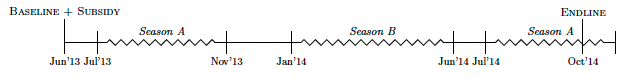
\includegraphics[width=0.8\linewidth]{"chapters/n2a_impact/figures/schedule.png"}
  \caption{Study timeline}
  \label{fig:n2a:timeline}
\end{figure}


To ensure that the NGOs’ relationships of mutual trust with communities were effectively leveraged, implementing partners for the input subsidy program were assigned to the villages in which they also had implemented the N2Africa extension services during the previous season. Local development committees (CLD) informed community members of the possibility to buy new inputs at a reduced price (75\% of the market price) and provided a delayed payback scheme, in which a deposit of 500 FC (0.54 USD) was required upfront and the remainder was owed after the next harvest. Participants were also offered the option to pay back in kind (seeds) instead of cash if preferred. Each implementing partner NGO customized six variations of input packages (each worth about 26 USD) that all contained a combination of improved seeds, fertilizer and (or) inoculant to best suit the preferences and needs of the local farmers. The value of the input packages of 26 USD is a significant amount compared to our estimate of the average household’s value of agricultural production (180 USD) for one season. The down payment on the other hand is very affordable to the average farmer. CLDs were responsible for registering community farmers and ordering the necessary packages. Agro-dealers delivered the ordered inputs to the communities before the start of the new 2013 planting season A, a month later. Inputs were delivered to the CLDs, who were then responsible for coordinating the distribution of the inputs to the respective buyers within the community and collecting the remaining payment owed after the harvest.

\section{Data}
Our research comprises 64 villages. The sampling frame was developed in collaboration with the implementing partners and required villages selected satisfy (i) that at least one of the implementing partners had established contacts within the community; (ii) that the village was accessible by motorized transport; and (iii) that the village had not participated in any N2Africa intervention previously, other than the extension program in the previous season.

Villages were randomly assigned to receiving the subsidy scheme or not, stratified within each axis. Data collection involved several steps (see Figure \ref{fig:n2a:timeline}). First, during June and July 2013, we administered a detailed household survey to 10 randomly selected households per village, comprising a sample of 521 households.\footnote{Interviews were conducted primarily in Swahili and data was recorded using ODK software on tablets.} In each household, the person most knowledgeable about agricultural activities was the primary respondent. In almost all cases (93\%) this was the head of household (56\%) or their spouse (37\%). In the remaining cases, other adult household members responded. In addition to the household interviews, community meetings were organized to collect information on proximity to markets and demographics. A year and a half later, in October 2014, we implemented a second round of surveys with the same households. The questionnaires included modules on demographics, housing, agriculture, food security, and social and formal financial support systems. A team of 37 enumerators, recruited with the assistance of the Catholic University of Bukavu (UCB), conducted the surveys and community meetings.


\begin{table}[hp] \centering
\newcolumntype{C}{>{\centering\arraybackslash}X}

\caption{Baseline descriptive statistics and balance}
\label{tab:n2a_impact:balance}
{\footnotesize
\begin{tabularx}{\textwidth}{lCCCCCCC}

\toprule
&{(1)}&{(2)}&{(3)}&{(4)}&{(5)}&{(6)}&{(7)} \tabularnewline
&\multicolumn{2}{c}{All}&\multicolumn{2}{c}{Treatment}&\multicolumn{2}{c}{Control}&{(4)-(6)}\tabularnewline
\tiny \tabularnewline
{}&{N}&{Mean}&{N}&{Mean}&{N}&{Mean}&{ } \tabularnewline
\midrule\addlinespace[1.5ex]
Inoculant knowledge&521&0.05&256&0.05&265&0.05&0.01 \tabularnewline
&&(0.22)&&(0.23)&&(0.22)& \tabularnewline
Fertilizer knowledge&521&0.94&256&0.93&265&0.95&-0.02 \tabularnewline
&&(0.24)&&(0.26)&&(0.22)& \tabularnewline
Inoculant Use&521&0.03&256&0.04&265&0.03&0.01 \tabularnewline
&&(0.18)&&(0.19)&&(0.16)& \tabularnewline
Fertilizer Use&521&0.03&256&0.03&265&0.03&0.00 \tabularnewline
&&(0.17)&&(0.17)&&(0.16)& \tabularnewline
Beans Yield&255&3.55&135&3.47&120&3.63&-0.16 \tabularnewline
&&(2.92)&&(2.91)&&(2.94)& \tabularnewline
Cassava Yield&383&7.71&175&7.65&208&7.77&-0.12 \tabularnewline
&&(1.78)&&(1.90)&&(1.67)& \tabularnewline
HFIAS Total&520&15.41&255&16.32&265&14.53&1.79** \tabularnewline
&&(6.49)&&(6.38)&&(6.49)& \tabularnewline
Female household head&521&0.13&256&0.14&265&0.12&0.02 \tabularnewline
&&(0.34)&&(0.35)&&(0.33)& \tabularnewline
Age household head&518&45.87&253&46.89&265&44.89&1.99 \tabularnewline
&&(15.40)&&(15.74)&&(15.04)& \tabularnewline
Level of education head (category)&519&1.46&255&1.32&264&1.60&-0.28 \tabularnewline
&&(1.47)&&(1.42)&&(1.51)& \tabularnewline
Household head born in village&521&0.62&256&0.59&265&0.64&-0.05 \tabularnewline
&&(0.49)&&(0.49)&&(0.48)& \tabularnewline
Primary occupation head is farmer&521&0.79&256&0.79&265&0.79&-0.00 \tabularnewline
&&(0.41)&&(0.41)&&(0.41)& \tabularnewline
Household size&521&6.68&256&6.57&265&6.78&-0.21 \tabularnewline
&&(2.72)&&(2.70)&&(2.74)& \tabularnewline
Household has a tin roof&521&0.52&256&0.53&265&0.52&0.01 \tabularnewline
&&(0.50)&&(0.50)&&(0.50)& \tabularnewline
Distance from input market (Km)&464&6.22&233&7.51&231&4.92&2.59 \tabularnewline
&&(7.61)&&(9.86)&&(3.90)& \tabularnewline
Tot. Val. Ag. Prod. (USD)&511&180.82&251&165.81&260&195.32&-29.52 \tabularnewline
&&(413.68)&&(408.09)&&(419.28)& \tabularnewline
Plot soil quality (wgtd average) &521&3.19&256&3.22&265&3.16&0.06 \tabularnewline
&&(1.04)&&(1.04)&&(1.04)& \tabularnewline
Plot ownership (wgtd average)&517&0.81&253&0.82&264&0.80&0.02 \tabularnewline
&&(0.37)&&(0.37)&&(0.37)& \tabularnewline
Grows leguminous crops (1=yes)&511&0.57&251&0.58&260&0.55&0.03 \tabularnewline
&&(0.50)&&(0.49)&&(0.50)& \tabularnewline
\bottomrule \addlinespace[1.5ex]

\end{tabularx}
\begin{flushleft}
\footnotesize Standard Deviations in parantheses; *p $<$ 0.1,**p $<$ 0.05,***p $<$ 0.01
\end{flushleft}
}
\end{table}


Variable definitions are given in Appendix Table \ref{tab:n2a_impact:vardef}, and descriptive statistics for the baseline survey are provided in Table \ref{tab:n2a_impact:balance}, which also compares mean values across the control and treatment (input subsidy) group. The first rows in Table \ref{tab:n2a_impact:balance} present baseline descriptive statistics for our outcome variables. Only three percent of households reported having used chemical fertilizer or inoculant in the previous season. Inputs provided in the subsidy program hence comprise new technologies for nearly all households in the sample. Yields for beans and cassava are log-transformed, with a value of on average 35kg/ha and 2230kg/ha respectively, and are comparable across treatment and control groups. Food insecurity is measured using the Household Food Insecurity Access Scale (HFIAS) \citep{Coates2007}. This scale measures food insecurity over three domains that capture different aspects of food insecurity: anxiety, quality and intake. We use the total HFIAS Score, which ranges from 0 to 27 with a higher score indicating greater food insecurity (see Table \ref{tab:n2a_impact:foodsecitems} in the Appendix for the survey questions that were used to construct the HFIAS Score). Reported insecurity is high throughout the sample, and we find that the input subsidy group was somewhat worse off than the control group in terms of food insecurity at baseline. 

Subsequent rows in Table \ref{tab:n2a_impact:balance} report a number of household characteristics. The household heads are predominantly male (only 13 percent of households have a female household head), around 46 years old, and mostly have some primary education. About 60 percent of the household heads were born in the village they currently live in, and about 80 percent of households identify agriculture as the household head’s primary occupation. Around half of the households have a tin roof. The average distance to an input market is 6.2 km, or more than one hour’s walk. The total value of the agricultural production is around 180 USD. The soil quality of the land on which they farm is rated 3.1 on a five-point scale, and the land is mostly owned by the households. Finally, about 60\% of the households grow legumes (soybeans, beans, or peanuts), the main type of crops to benefit from inoculant, while only about five percent of household correctly identify on which crops to use inoculant. Almost all households correctly indicate the type of fertilizer to apply to legumes.\footnote{We unfortunately have no data on knowledge of the benefits of inoculant or fertilizer and hence we are not able to analyze whether the subsidy program affected perceived benefits (which may be a relevant channel for persistent impacts on use). We only know, based a qualitative analysis of the extension and input subsidy program combined \citep{Kendzior2015}, that farmers across several villages noticed a positive effect of inoculant on soy yields in extension demonstration plots (they mentioned earlier germination, more and bigger pods). Fertilizer was not used by many farmers, but farmers who did use it applied it to small plots planted with more valuable crops, suggesting they were aware of the positive effect on yields.}

Apart from baseline food insecurity, there are no significant differences in baseline characteristics between treatment and control households. We control for the baseline HFIAS Score in all of the following analyses.

\subsection{Attrition}
During data collection, measures were taken to minimize household and village level attrition. At the village level there was no attrition. Within each village, enumerators announced the arrival of the research team one day in advance to ensure that all targeted households were present during the scheduled enumerator visits. For those instances where households were not present on the scheduled visit, a second date was scheduled to interview any missing households. Despite these measures, in both treatment arms, 23\% of the households that were part of the first round could not be reached during the second round of data collection (see column 1 in Appendix Table \ref{tab:n2aimpact:attr}). To some extent, this is to be expected given the post-conflict setting where displacement is typically high. In the second column of Table \ref{tab:n2aimpact:attr}, we analyze whether any baseline characteristics are predictive of differential attrition across treatment arms. We find no evidence of differential attrition, except for baseline total value of farm outputs. However, the coefficient is small: for a 10\% increase in agricultural production, the probability of a treatment group household dropping out of our sample increases by 0.2\% relative to control, a negligible difference. 

\section{Empirical strategy} 
We assess the impacts of offering the subsidy intervention use of inoculant and fertilizer, yields, and food security relative to a condition where famers only receive the N2Africa extension program.  Specifically, we use OLS to estimate:

\begin{equation}
	\label{eq:n2a:basic}
	Y_{ijt}=\alpha+{\beta Subsidy}_j+{\delta\ Y}_{ij,t-1}+\ \gamma X_{ij,t-1}+\ \Gamma A_k+\varepsilon_{ijt}
\end{equation}

Where $Y_{ijt}$ is the outcome measure for respondent $i$, in village $j$, in the second round of data collection. ${Subsidy}_j$ is a dummy that takes value 1 if village $j$ was randomly selected to receive access to subsidized inputs, $Y_{ijt-1}$ is the outcome measure at baseline (included to increase precision), $X_{ij,t-1}$ is baseline food insecurity, $A_k$ is the stratum (axis) fixed effect, and $\varepsilon_{ijt}$ is the error term. In all models, we cluster standard errors at the village level. Coefficient $\beta$ captures the intent to treat effect (ITT) of offering the subsidy scheme.\footnote{We conducted a short follow-up study in September 2013 to assess take-up and check whether inputs had been (timely) delivered.  Due to reasons of increased insecurity this survey was not conducted well and take-up rates were only recorded in 20\% of our sample. We therefore only report IIT impacts here. }

In addition, we explore how the input subsidy intervention differentially affected households stratified across several dimensions. Understanding such heterogeneous impacts can provide key descriptive insights for future exploration to tailor policy towards particularly responsive households in order to improve project effectiveness. Second, heterogeneous treatment effects can elucidate key drivers and constraints to intervention effectiveness within the sample. Of particular interest in our sample are distance to input markets (an indicator for distance greater than 5 km, which is the median), land ownership (an indicator for whether the household owns any of their land), and the gender and education level of household heads (education is measured by an indicator for whether the household head has at least primary education). We also consider village size, which varies between 40 and 740 households, to capture the impact of the extension services offered before the subsidy intervention (it is likely that in larger villages, a smaller fraction of farmers was trained directly and by the lead farmers). To this end, we generate a dummy variable that indicates whether the number of households in the village is greater than the median (138 households). We re-run model (\ref{eq:n2a:basic}) and include a level and interaction term for $H_{ij}$, the vector of subgroup indicators. Specifically, we estimate:

\begin{equation}
\label{eq:n2a:hte}
Y_{ijt}=\alpha+{\beta Subsidy}_j+\ \gamma X_{it-1}+{\delta\ Y}_{ijt-1}+\pi\ H_{ij}\ast{Subsidy}_j+\theta H_{ij}+\ \Gamma A_k+\varepsilon_{ijt}
\end{equation}

All symbols are the same as above, and coefficient estimates $\pi$ capture differences in the intent to treat effect of the input subsidy intervention on outcomes between relevant subgroups.

\section{Results}
\todo{ERWIN: je bespreekt ITT effects, misschien een voetnoot over LATE toevoegen (als de first stage werkt; uptake is natuurlijk laag...)}

\todo{ERWIN: je noemt "low power" als een probleem. Lijkt me terecht. Je zou een voetnoot kunnen toevoegen met een opmerking gebaseerd op een ex-post power analyse: wat is de MDE voor je belangrijkste variabele? Volgens mij is dat gewoon 2.8 keer de SE die je geschat hebt, dus dit is zo gepiept. Vervolgens kun je iets zeggen over de MDE: is het aannemelijk dat dit effect op zou kunnen treden, in het licht van je interventie zo ja; dan ben je niet echt under-powered, wellicht).}


In Table \ref{tab:n2aimpact:main} we show the estimated effects of offering the subsidy program on farmers’ use of fertilizer and inoculant, production (yields) of cassava and beans, and food security. The effects on input use (columns 1-2) are positive and statistically significant, and also indicate economically meaningful effects of the subsidy program. Inoculant use increased by three percentage points, compared to the control group mean of one percent (column 1) and fertilizer use increased by more than five percentage points compared to the control group mean of three percent (column 2). These results are obtained one year (that is, two agricultural seasons) after farmers were offered the subsidy, suggesting effects on input use are persistent.\footnote{We unfortunately lack data on when farmers started using the inputs and where they obtained them. It is technically possible that farmers purchased subsidized inputs and started using them only two seasons later, and therefore the treatment effect need not capture persistence of input use. This seems unlikely, however, and we believe a more plausible story is that farmers bought inputs during the subsidy period and have continued their use in the following seasons by purchasing them unsubsidized. This is corroborated by our heterogeneity results, which show the subsidy treatment had no effect on input use in villages located far away from input markets.} The findings are consistent with those by \cite{Carter2014}, who find fertilizer use remains significantly higher two years after a subsidy was provided. 

%e1 contains a few tweaks: text size is set to small, and the column type of the notes was changed. 
\begin{table}[htbp]\centering \small
\def\sym#1{\ifmmode^{#1}\else\(^{#1}\)\fi}
\caption{Knowledge, input use, yield, and food security \label{tab:n2aimpact:main}}
\begin{tabular}{l*{7}{c}}
\toprule
                    &\multicolumn{1}{c}{(1)}&\multicolumn{1}{c}{(2)}&\multicolumn{1}{c}{(3)}&\multicolumn{1}{c}{(4)}&\multicolumn{1}{c}{(5)}&\multicolumn{1}{c}{(6)}&\multicolumn{1}{c}{(7)}\\
                    &\multicolumn{1}{c}{\specialcell{Inoculant\\knowledge}}&\multicolumn{1}{c}{\specialcell{Fertilizer\\knowledge}}&\multicolumn{1}{c}{\specialcell{Inoculant\\use}}&\multicolumn{1}{c}{\specialcell{Fertilizer\\Use}}&\multicolumn{1}{c}{\specialcell{Beans\\Yield}}&\multicolumn{1}{c}{\specialcell{Casava\\Yield}}&\multicolumn{1}{c}{\specialcell{HFIAS\\Score}}\\
\midrule
Subsidy             &      0.0391         &      0.0165         &      0.0301\sym{**} &      0.0513\sym{**} &       0.140         &      -0.175         &       0.845         \\
                    &    (0.0235)         &    (0.0227)         &    (0.0127)         &    (0.0209)         &     (0.444)         &     (0.313)         &     (0.777)         \\
\addlinespace
Lagged dep. var.    &       0.248\sym{***}&     -0.0263         &       0.211\sym{**} &       0.208\sym{*}  &      0.0593         &     0.00364         &       0.233\sym{***}\\
                    &    (0.0932)         &    (0.0293)         &    (0.0936)         &     (0.118)         &    (0.0804)         &    (0.0496)         &    (0.0580)         \\
\midrule
N                   &         520         &         520         &         520         &         520         &         167         &         270         &         512         \\
Mean Control Group  &        0.06         &        0.93         &        0.01         &        0.03         &        5.06         &        7.72         &       14.10         \\
SD Control Group    &        0.25         &        0.25         &        0.09         &        0.18         &        2.38         &        1.94         &        6.90         \\
No. clusters        &          64         &          64         &          64         &          64         &          54         &          61         &          64         \\
\bottomrule
\multicolumn{8}{p\textwidth}{\footnotesize * p$<$0.10, ** p$<$0.05, *** p$<$0.01; Standard errors clustered at the village level in parentheses; controls include stratum fixed effect and baseline levels of food insecurity.}\\
\end{tabular}
\end{table}


However, we find no evidence that this increased adoption of inoculant and fertilizer translates into better yields or improved food security (Table \ref{tab:n2aimpact:main}, columns 3-5), contrasting work by \cite{Carter2014} and \cite{Brune2016}. The point estimates are small and statistically insignificant. The absence of effects on yields and food security may be due to low statistical power and a low overall absolute increase in input use. Given that less than 10 percent in our sample uses fertilizer and (or) inoculant, any potential treatment effects on yield and food security through the channel of increased input use would have to come from this very small group.
We run additional tests to see whether the specification we used affects the null-result on yields and food security. In particular, we check whether the high number of missing values for yields has an impact on our findings. In Appendix Table \ref{tab:n2aimpact:robust} (column 1) we estimate the effect of treatment on the value of total agricultural output, by multiplying the output of each crop with the average selling price reported by farmers in our sample. This measure is available for all farmers in the estimation sample, and will capture changes in production, regardless of the type of crops grown.\footnote{Since we use the average crop price reported in the sample, any differences between treatment and control group {}in the value of output will be due to differences in output quantity, rather than prices.} The coefficient is small and statistically insignificant, so similar to the results for beans and cassava yields, hence we find no evidence that the subsidy program affected farmers’ total output. Next, given the high level of food insecurity among the study sample, we estimate the effect of treatment on the prevalence of severe food insecurity in column 2 of Table \ref{tab:n2aimpact:robust}, using a logit model. In defining severe food insecurity, we follow the categorization of \cite{Coates2007}. We find no statistically significant effect of subsidies on the prevalence of severe food insecurity, supporting the main result that food security was not affected.

\begin{table}[htbp]\centering
\def\sym#1{\ifmmode^{#1}\else\(^{#1}\)\fi}
\caption{Heterogeneous Effects \label{tab:n2aimpact:hte}}
\begin{tabular}{l*{7}{c}}
\hline\hline
                    &\multicolumn{1}{c}{(1)}&\multicolumn{1}{c}{(2)}&\multicolumn{1}{c}{(3)}&\multicolumn{1}{c}{(4)}&\multicolumn{1}{c}{(5)}&\multicolumn{1}{c}{(6)}&\multicolumn{1}{c}{(7)}\\
                    &\multicolumn{1}{c}{\specialcell{Inoculant\\knowledge}}&\multicolumn{1}{c}{\specialcell{Fertilizer\\knowledge}}&\multicolumn{1}{c}{\specialcell{Inoculant\\use}}&\multicolumn{1}{c}{\specialcell{Fertilizer\\Use}}&\multicolumn{1}{c}{\specialcell{Beans\\Yield}}&\multicolumn{1}{c}{\specialcell{Casava\\Yield}}&\multicolumn{1}{c}{\specialcell{HFIAS\\Score}}\\
\hline
Subsidy             &      0.0197         &      0.0401         &      0.0614\sym{*}  &      0.0492         &       1.223         &      -1.499         &       1.166         \\
                    &    (0.0543)         &    (0.0478)         &    (0.0331)         &    (0.0536)         &     (1.303)         &     (1.178)         &     (1.618)         \\
[1em]
Primary education * subsidy&      0.0379         &     -0.0411         &     -0.0162         &     -0.0179         &       0.311         &     -0.0199         &       0.657         \\
                    &    (0.0537)         &    (0.0477)         &    (0.0316)         &    (0.0494)         &     (0.831)         &     (0.677)         &     (1.405)         \\
[1em]
Market dist. $>$ 5km * subsidy&     -0.0225         &     -0.0340         &     -0.0758\sym{***}&     -0.0507         &     -0.0671         &       0.445         &       0.326         \\
                    &    (0.0455)         &    (0.0408)         &    (0.0273)         &    (0.0439)         &     (1.045)         &     (0.856)         &     (1.700)         \\
[1em]
Owns land * subsidy &      0.0677         &      0.0150         &      0.0205         &      0.0449         &      -1.042         &       1.388         &      -2.221         \\
                    &    (0.0481)         &    (0.0376)         &    (0.0305)         &    (0.0457)         &     (1.114)         &     (0.874)         &     (1.578)         \\
[1em]
Female head * subsidy&     -0.0395         &     -0.0233         &     0.00511         &      0.0576         &       1.267         &       0.481         &      -0.809         \\
                    &    (0.0707)         &    (0.0486)         &    (0.0354)         &    (0.0818)         &     (1.136)         &     (0.759)         &     (1.887)         \\
[1em]
Village size $>$ 138 * subsidy&     -0.0474         &    -0.00170         &     -0.0204         &     -0.0120         &      -0.959         &       0.457         &       1.218         \\
                    &    (0.0549)         &    (0.0521)         &    (0.0269)         &    (0.0479)         &     (0.998)         &     (0.708)         &     (1.679)         \\
[1em]
Lagged dep. var.    &       0.265\sym{***}&     -0.0516\sym{***}&       0.205\sym{**} &       0.232\sym{*}  &      0.0771         &     0.00560         &       0.211\sym{***}\\
                    &    (0.0968)         &    (0.0164)         &    (0.0922)         &     (0.124)         &    (0.0763)         &    (0.0652)         &    (0.0647)         \\
\hline
N                   &         439         &         439         &         439         &         439         &         160         &         230         &         439         \\
Mean Control Group  &        0.07         &        0.94         &        0.00         &        0.03         &        5.05         &        7.61         &       14.35         \\
SD Control Group    &        0.26         &        0.24         &        0.07         &        0.16         &        2.42         &        2.08         &        6.75         \\
No. clusters        &          56         &          56         &          56         &          56         &          49         &          53         &          56         \\
\hline\hline
\multicolumn{8}{l}{\footnotesize * p$<$0.10, ** p$<$0.05, *** p$<$0.01; Standard errors clustered at the village level in parentheses; controls include stratum fixed effect and baseline levels of food insecurity.}\\
\end{tabular}
\end{table}


\subsection{Heterogeneity}
In order to reveal potential underlying mechanisms driving the results, we assess whether the input subsidy scheme had differential impacts among varying sub-groups of participants effects (Table \ref{tab:n2aimpact:hte}).\footnote{Note that because of missing values for some of the variables (see sample sizes in Table \ref{tab:n2a_impact:balance}), the sample in the heterogeneity analysis (Table \ref{tab:n2aimpact:hte}) is smaller than sample in our main analysis (Table \ref{tab:n2aimpact:main}).} We analyze heterogeneity by education and gender of the household head, distance to input markets, land ownership, and size of the village. 

Overall, we find no evidence of treatment heterogeneity, except for distance to an input market. The impact of the subsidy scheme on input use is smaller in households that are further away from input markets. The interaction effect is negative and statistically significant for inoculant use, while it is not statistically significant for fertilizer use. In fact, for both inputs, the (negative) interaction effect is somewhat larger in magnitude than the main effect of treatment, suggesting that both fertilizer use and inoculant use were not affected in households located more than 5km from an input market. This finding also supports the notion that farmers did not “save” the subsidized inputs only to be used two seasons later, but rather that our overall impact captures persistent usage, which was driven by those farmers that live close enough to input markets. This further suggests that the (time and financial) costs associated with accessing inputs appear as a barrier to a persistent impact of input subsidies on input use. 

\subsection{Spillovers}
Identification of treatment effects rests on the assumption of non-interference. It is possible, however, that the subsidy scheme affected households in control villages. For example, the subsidized input packages could have been shared between treatment and control households. In this case, the estimates in Table \ref{tab:n2aimpact:main} provide a lower bound of the true treatment effects. To assess whether our main findings are robust to potential spillovers, we estimate equation (1) again, adding an indicator for being within 1 km of a subsidy treatment village (the coefficient on this indicator can be interpreted as an upper bound on spillovers, as we are unlikely to find any spillovers at larger distances if we do not find any within 1km). Table \ref{tab:n2aimpact:spill} presents the results. Our main findings on input use are not affected by spillovers: the effect of the subsidy scheme on inoculant and fertilizer use (columns 1 and 2) is still significantly positive and very similar to the main estimates in Table \ref{tab:n2aimpact:main}. There is also no indication of spillovers in terms of yields and food security.

\section{Discussion and conclusions} 
Smallholder agriculture in much of sub-Saharan Africa is severely constrained. Poorly functioning input, output and credit markets and low quality infrastructure inhibit growth in the agricultural sector. Input subsidies, while long regarded as inefficient and misused for political gains, have regained popularity as a possibly effective tool to increase access to inputs among rural farm households. We study the causal effect of offering input subsidies on input use, yields, and food security, in a fragile and conflict-prone setting where in- and output markets are sparse, and input use prior to the intervention is extremely low. 
Our results suggest that the intervention was successful in increasing use of two important yields enhancing inputs: a new technology called inoculant and chemical fertilizer. In our sample, reported input use nearly doubles, corresponding with findings elsewhere \citep{Carter2014,Brune2016}. In addition, we find that only villages relatively close to input markets are likely to benefit from the subsidy scheme: input use two seasons after the subsidy was provided is not affected in villages located at above-median distance from input markets. This suggests that access to markets is a key constraint to raising adoption. Unfortunately, we do not find that increases in input use translate into increases in yields and food security, but the lack of impact may be due to limited power in our sample and to a low absolute impact on input use. Taken together, our results caution against overoptimistic views on the downstream effects of productivity enhancing technologies. Perhaps, larger interventions that target fundamental changes in market structure and access are required in order to develop local supply chains and thus structurally lower the costs of inputs. This might raise input use to a level where increases in yields and subsequent food security may be realized. 
There are three caveats to our study. First, and unfortunately, we do not have reliable data on actual take-up of the treatment (i.e. the purchase of subsidized input packages) within villages, which would allow for estimating local average effects among adopters. Program implementation in DRC takes place under challenging conditions and recording of activities and key process indicators (such as who within each community ordered input packages) was incomplete. We only know whether farmers in treatment villages use these inputs two seasons after the subsidy was provided. Second, our design does not assess the impact of extension services or subsidies alone and hence cannot provide insight in to what binding constraint, i.e. information or input subsidies, would make the largest contribution to raising smallholder agricultural productivity. Finally, we have no information on whether the subsidy had an effect on input use at the intensive margin, which is an important dimension especially to understand how interventions may impact yields and food security. This is left for future work. 


\clearpage
\section{Appendix}
\setcounter{table}{0}
\renewcommand{\thetable}{\arabic{chapter}.A\arabic{table}}





\begin{table}[htbp]
	\scriptsize
	\caption{Variable Definitions}
	\label{tab:n2a_impact:vardef}
	\bgroup
	\def\arraystretch{1.3}
    \begin{tabular}{p{0.3\textwidth}p{0.6\textwidth}}
    \toprule
	
	\multicolumn{2}{l}{\textit{Outcome Indicators}}\\
	\midrule
	Inoculant use & 1= household uses inoculant, 0=otherwise\\
	Fertilizer use & 1= household uses fertilizer, 0=otherwise\\
	Log beans yield (in Kg/ha) & Beans harvested (kg) divided by the surface (ha), log transformed\\
	Log cassava yield (in Kg/ha) & Cassava harvested (kg) divided by surface (ha), log transformed\\
	HFIAS Score & Food security indicator, ranging from 0 (least food insecurity) to 27 (most food insecurity). See Table A5 for more information\\
	\multicolumn{2}{l}{\textit{Other variables}}\\
	\midrule
	Female household head & 1= household head is female, 0=otherwise\\
	Age household head  & Age of the head of the household in years \\
	Education level household head & 0= No education, 1= Some primary, 2= Primary Complete, 3= Some secondary, 4= Secondary complete, 5= Higher education, 6= Professional education\\
	Household head born in village & 1= household head was born in the village, 0=otherwise\\
	Head primary occupation farmer & 1= household head primary occupation is a farmer, 0=otherwise\\
	Household size & Total number of people living in the household\\
	House has tin roof & 1= household roof construction material is tin, 0=otherwise\\
	Distance from input market & Distance from input market, in km\\
	Value agricultural production & Total production of all crops, multiplied by the average price, in USD\\
	Plot soil quality  & Average self-reported soil quality of agricultural plots cultivated (weighted by plot size). 1 = “Very infertile”, 2= “Infertile”, 3= “Normal”, 4= “Fertile”, 5 = “Very Fertile”\\
	Plot ownership & Average ownership status of agricultural plots cultivated (weighted by plot size), where: 1= “Owned”, 0 = “Not owned”\\
	Grows leguminous crops & 1 = household grows any leguminous crops, 0= otherwise\\
	Inoculant knowledge  & 1= household knows on which crops to use inoculant (leguminous crops), 0=otherwise\\
	Fertilizer knowledge  & 1= respondent answers correctly that nitrogen fertilizer is not needed on leguminous crops, 0=otherwise\\
	HFIAS: Severely Food Insecure & 1 = Severely food insecure; 0 = Food secure, mildly food insecure, or moderately food insecure. See Table A5 for more information\\


    \bottomrule
    \end{tabular}%
    \egroup
\end{table}%

\begin{table}[htbp]\centering
\def\sym#1{\ifmmode^{#1}\else\(^{#1}\)\fi}
\caption{Correlates of Attrition \label{tab:n2aimpact:attr}}
\begin{tabular}{l*{2}{c}}
\hline\hline
                    &\multicolumn{1}{c}{(1)}   &\multicolumn{1}{c}{(2)}   \\
                    &   Attrition   &   Attrition   \\
\hline
Subsidy             &      -0.005   &      -0.013   \\
                    &     (0.059)   &     (0.203)   \\
Treatment * Female household head&               &       0.078   \\
                    &               &     (0.098)   \\
Treatment * Age household head&               &      -0.000   \\
                    &               &     (0.002)   \\
Treatment * Level of education head (category)&               &       0.026   \\
                    &               &     (0.023)   \\
Treatment * Household head born in village&               &       0.011   \\
                    &               &     (0.071)   \\
Treatment * Primary occupation head is farmer&               &       0.058   \\
                    &               &     (0.081)   \\
Treatment * Household size&               &      -0.005   \\
                    &               &     (0.012)   \\
Treatment * Household has a tin roof&               &      -0.025   \\
                    &               &     (0.070)   \\
Treatment * Distance from input market (Km)&               &      -0.007   \\
                    &               &     (0.005)   \\
Treatment * Log of Total Value Agr. Production (USD)&               &       0.023*  \\
                    &               &     (0.013)   \\
Treatment * Plot soil quality (wgtd average) &               &      -0.004   \\
                    &               &     (0.033)   \\
Treatment * Plot ownership (wgtd average)&               &      -0.109   \\
                    &               &     (0.085)   \\
Treatment * Grows leguminous crops (1=yes)&               &       0.015   \\
                    &               &     (0.070)   \\
Treatment * block==Ouest (Bukavu - Mwenga)&               &       0.037   \\
                    &               &     (0.095)   \\
Treatment * block==Sud (Bukavu - Uvira)&               &      -0.048   \\
                    &               &     (0.124)   \\
Constant            &       0.230***&       0.332*  \\
                    &     (0.043)   &     (0.170)   \\
\hline
Observations        &         674   &         530   \\
No. clusters        &          69   &          56   \\
\hline\hline
\multicolumn{3}{l}{\footnotesize Notes: * p$<$0.10, ** p$<$0.05, *** p$<$0.01; Standard errors clustered at the village level in parentheses.}\\
\end{tabular}
\end{table}


\begin{table}[htbp]\centering
\def\sym#1{\ifmmode^{#1}\else\(^{#1}\)\fi}
\caption{Robustness Checks on Yields and Food Security \label{tab:n2aimpact:robust}}
\begin{tabular}{l*{2}{c}}
\hline\hline
                    &\multicolumn{1}{c}{(1)}&\multicolumn{1}{c}{(2)}\\
                    &\multicolumn{1}{c}{\specialcell{Log Total Value Agr.\\Production (USD)}}&\multicolumn{1}{c}{\specialcell{HFIAS: Severely Food\\Insecure}}\\
\hline
Subsidy             &      -21.50         &      0.0379         \\
                    &     (24.97)         &    (0.0538)         \\
[1em]
Lagged dep. var.    &       0.100\sym{*}  &      0.0715         \\
                    &    (0.0575)         &    (0.0515)         \\
\hline
N                   &         520         &         512         \\
Mean Control Group  &      142.59         &        0.69         \\
SD Control Group    &      336.11         &        0.46         \\
No. clusters        &          64         &          64         \\
\hline\hline
\multicolumn{3}{l}{\footnotesize * p$<$0.10, ** p$<$0.05, *** p$<$0.01; Standard errors clustered at the village level in parentheses; controls include stratum fixed effect and baseline levels of food insecurity. Marginal effects (at means) for a logit regression are reported column 2}\\
\end{tabular}
\end{table}

\begin{table}[htbp]\centering \small
\def\sym#1{\ifmmode^{#1}\else\(^{#1}\)\fi}
\caption{Spillover analysis \label{tab:n2aimpact:spill}}
\begin{tabular}{l*{7}{c}}
\hline\hline
                    &\multicolumn{1}{c}{(1)}&\multicolumn{1}{c}{(2)}&\multicolumn{1}{c}{(3)}&\multicolumn{1}{c}{(4)}&\multicolumn{1}{c}{(5)}&\multicolumn{1}{c}{(6)}&\multicolumn{1}{c}{(7)}\\
                    &\multicolumn{1}{c}{\specialcell{Inoculant\\knowledge}}&\multicolumn{1}{c}{\specialcell{Fertilizer\\knowledge}}&\multicolumn{1}{c}{\specialcell{Inoculant\\use}}&\multicolumn{1}{c}{\specialcell{Fertilizer\\Use}}&\multicolumn{1}{c}{\specialcell{Beans\\Yield}}&\multicolumn{1}{c}{\specialcell{Casava\\Yield}}&\multicolumn{1}{c}{\specialcell{HFIAS\\Score}}\\
\hline
Subsidy             &      0.0527\sym{**} &      0.0211         &      0.0315\sym{**} &      0.0558\sym{**} &       0.152         &      -0.245         &       0.789         \\
                    &    (0.0250)         &    (0.0282)         &    (0.0155)         &    (0.0246)         &     (0.444)         &     (0.299)         &     (0.956)         \\
[1em]
Subsidy $<$1km      &      0.0415         &      0.0143         &     0.00420         &      0.0139         &      0.0701         &      -0.197         &      -0.173         \\
                    &    (0.0428)         &    (0.0471)         &    (0.0120)         &    (0.0258)         &     (0.786)         &     (0.480)         &     (1.157)         \\
[1em]
Lagged dep. var.    &       0.244\sym{***}&     -0.0287         &       0.212\sym{**} &       0.209\sym{*}  &      0.0601         &     0.00405         &       0.234\sym{***}\\
                    &    (0.0893)         &    (0.0301)         &    (0.0937)         &     (0.118)         &    (0.0821)         &    (0.0498)         &    (0.0578)         \\
\hline
N                   &         520         &         520         &         520         &         520         &         167         &         270         &         512         \\
Mean Control Group  &        0.06         &        0.93         &        0.01         &        0.03         &        5.06         &        7.72         &       14.10         \\
SD Control Group    &        0.25         &        0.25         &        0.09         &        0.18         &        2.38         &        1.94         &        6.90         \\
No. clusters        &          64         &          64         &          64         &          64         &          54         &          61         &          64         \\
\hline\hline
\multicolumn{8}{p\textwidth}{\footnotesize * p$<$0.10, ** p$<$0.05, *** p$<$0.01; Standard errors clustered at the village level in parentheses; controls include stratum fixed effect and baseline levels of food insecurity.}\\
\end{tabular}
\end{table}



\begin{table}[htbp]
	\scriptsize
	\caption{Food insecurity items}
	\label{tab:n2a_impact:foodsecitems}
	\bgroup
	\def\arraystretch{1.3}
    \begin{tabular}{p{0.85\textwidth}p{0.05\textwidth}}
    \toprule
	
    \textbf{In the past four weeks}, & \textbf{Domain}\\
    \midrule
	1.    Did you worry that your household would not have enough food? & Anxiety\\
	2.    In the past four weeks, were you or any household member not able to eat the kinds of foods you preferred because of a lack of resources? & Quality\\
	3.    Did you or any household member have to eat a limited variety of foods due to a lack of resources? & Quality\\
	4.    Did you or any household member have to eat some foods that you really did not want to eat because of a lack of resources to obtain other types of food? & Quality\\
	5.    Did you or any household member have to eat a smaller meal than you felt you needed because there was not enough food? & Intake\\
	6.    Did you or any other household member have to eat fewer meals in a day because there was not enough food? & Intake\\
	7.    Was there ever no food to eat of any kind in your household because of lack of resources to get food? & Intake\\
	8.    Did you or any household member go to sleep at night hungry because there was not enough food? & Intake\\
	9.    Did you or any household member go a whole day and night without eating anything because there was not enough food? & Intake\\

    \midrule
    \multicolumn{2}{p\textwidth}{These questions are part of the Household Food Insecurity Access Scale (HFIAS), developed by the Food and Nutrition Technical Assistance Project (FANTA) (see Coates et al., 2007). For each item we asked households to indicate whether they occurred during the past four weeks (yes or no), and how often (1 = once or twice; 2 = three to ten times; 3 = more than ten times). The answers were combined into a single score for each item, indicating the frequency of occurrence in the past four week (0 = never; 1 = once or twice; 2 = three to ten times; 3 = more than ten times). The total HFIAS Score is calculated as the sum of all nine scores. Furthermore, we follow Coates et al (2007) in using these questions to categorize households in four categories, ranging from Food Secure to Severely Food Insecure.}\\
    \bottomrule
    \end{tabular}%
    \egroup
\end{table}%


%These questions are part of the Household Food Insecurity Access Scale (HFIAS), developed by the Food and Nutrition Technical Assistance Project (FANTA) (see Coates et al., 2007). For each item we asked households to indicate whether they occurred during the past four weeks (yes or no), and how often (1 = once or twice; 2 = three to ten times; 3 = more than ten times). The answers were combined into a single score for each item, indicating the frequency of occurrence in the past four week (0 = never; 1 = once or twice; 2 = three to ten times; 3 = more than ten times). The total HFIAS Score is calculated as the sum of all nine scores. Furthermore, we follow Coates et al (2007) in using these questions to categorize households in four categories, ranging from Food Secure to Severely Food Insecure.


\clearpage 
\bibliographystyle{chicago}
%path to .bib file (e.g. automatically exported by mendeley) DO NOT include the file extension!
\bibliography{tex_helpers/Thesis}